%%%%%%%%%%%%%%%%%%%%%%%%%%%%%%%%%%%%%%%%%%  不使用 authblk 包制作标题  %%%%%%%%%%%%%%%%%%%%%%%%%%%%%%%%%%%%%%%%%%%%%%
%-------------------------------PPT Title-------------------------------------
\title{02-\rm{Hartree-Fock}与\rm{DFT}}
%-----------------------------------------------------------------------------

%----------------------------Author & Date------------------------------------
%\author[\textrm{Jun\_Jiang}]{姜\;\;骏\inst{}} %[]{} (optional, use only with lots of authors)
%% - Give the names in the same order as the appear in the paper.
%% - Use the \inst{?} command only if the authors have different
%%   affiliation.
\institute[BCC]{\inst{}%
%\institute[Gain~Strong]{\inst{}%
\vskip -20pt 北京市计算中心}
%\vskip -20pt {\large 格致斯创~科技}}
\date[\today] % (optional, should be abbreviation of conference name)
{%	{\fontsize{6.2pt}{4.2pt}\selectfont{\textcolor{blue}{E-mail:~}\url{jiangjun@bcc.ac.cn}}}
\vskip 45 pt {\fontsize{8.2pt}{6.2pt}\selectfont{%清华大学\;\;物理系% 报告地点
	\vskip 5 pt \textrm{2022.07.01}}}
}

%% - Either use conference name or its abbreviation
%% - Not really information to the audience, more for people (including
%%   yourself) who are reading the slides onlin%%   yourself) who are reading the slides onlin%%   yourself) who are reading the slides onlineee
%%%%%%%%%%%%%%%%%%%%%%%%%%%%%%%%%%%%%%%%%%%%%%%%%%%%%%%%%%%%%%%%%%%%%%%%%%%%%%%%%%%%%%%%%%%%%%%%%%%%%%%%%%%%%%%%%%%%%

\subject{}
% This is only inserted into the PDF information catalog. Can be left
% out.
%\maketitle
\frame
{
%	\frametitle{\fontsize{9.5pt}{5.2pt}\selectfont{\textcolor{orange}{“高通量并发式材料计算算法与软件”年度检查}}}
\titlepage
}
%-----------------------------------------------------------------------------

%------------------------------------------------------------------------------列出全文 outline ---------------------------------------------------------------------------------
%\section*{}
%\frame[allowframebreaks]
%{
%  \frametitle{Outline}
%%  \frametitle{\textcolor{mycolor}{\secname}}
%  \tableofcontents%[current,currentsection,currentsubsection]
%}
%%在每个section之前列出全部Outline
%%类似的在每个subsection之前列出全部Outline是\AtBeginSubsection[]
%\AtBeginSection[]
%{
%  \frame<handout:0>%[allowframebreaks]
%  {
%    \frametitle{Outline}
%%全部Outline中,本部分加亮
%    \tableofcontents[current,currentsection]
%  }
%}

%-----------------------------------------------PPT main Body------------------------------------------------------------------------------------
\small
\section{\rm{Hartree-Fock~}方法}
\frame
{
	\frametitle{\textrm{Born-Oppenheimer~}近似}
	\begin{itemize}
		\item 由于原子核的质量要比电子大很多(一般要大3-4个数量级),在同样的相互作用下,原子核的运动比电子也慢得多
		\item 电子在每一时刻仿佛运动在静止原子核构成的势场中,而原子核运动时则感受不到电子的具体位置,感受到的是运动电子的平均作用力
		\item 可近似将原子核坐标与电子坐标变量分离,使得求解整个体系的波函数的复杂过程分解为求解电子波函数和求解原子核波函数两个相对简单的过程\\
			电子运动方程$$\hat{\mathbf H}_{\mathrm e}(\vec r,\vec{\mathbf R})\Psi(\vec r,\vec{\mathbf R})=E_{\mathrm e}(\vec{\mathbf R})\Psi(\vec r,\vec{\mathbf R})$$
			原子核运动方程$$[\hat{\mathbf T}_{\mathrm{nul}}+E_{\mathrm e}(\vec{\mathbf R})]\chi(\vec{\mathbf R})=E\chi(\vec{\mathbf R})$$
	\end{itemize}
}

\frame
{
	\frametitle{独立粒子近似}
	\textrm{n-}粒子体系中的每个粒子的运动,完全忽略粒子间的瞬时相互作用,认为第$i$个粒子在其余$\mathrm{n}-1$个粒子组成的平均势场中运动
	$$\Psi(\vec r_1,\vec r_2,\vec r_3,\cdots,\vec r_n)=\psi_1(\vec r_1)\psi_2(\vec r_2)\psi_3(\vec r_3)\cdots\psi_n(\vec r_n)$$
	$$\hat{\mathbf H}=\sum_{i=1}^N-\dfrac{1}{2}\nabla_i^2+\sum_{i=1}^NV_i(\vec r_i)+\sum_{i,j(j\neq i)}\dfrac{e^2}{|\vec r_i-\vec r_j|}$$
	粒子$i$的\textrm{Hartree}算符
	$$\hat{\mathbf h}_i=-\dfrac{1}{2}\nabla_i^2+V_i(r_i)+\sum_{j(j\neq i)}^N\dfrac{e^2}{|\vec r_i-\vec r_j|}$$
	因此每个粒子的运动方程为:
	$$\hat{\mathbf h}_i\psi_i(\vec r)=\bigg[-\dfrac{1}{2}\nabla_i^2+V_i(r_i)+\sum_{j(j\neq i)}^N\dfrac{e^2}{|\vec r_i-\vec r_j|}\bigg]\psi_i(\vec r)=\varepsilon\psi_i(\vec r)$$ 
}

\frame
{
	\frametitle{\textrm{Slater~}行列式}
	简单乘积的独立粒子波函数不满足全同粒子置换对称性要求,不能正确表示电子不可辨认的物理属性
	
	\textrm{Slater}建议用行列式形式表示具有反对称性的波函数
	\begin{displaymath}
		\hspace*{-10pt}\Psi(\vec r_1,\vec r_2,\vec r_3,\cdots,\vec r_n)=\dfrac1{\sqrt{n!}}
		\left|\begin{array}{ccccc}
			\psi_1(\vec r_1)&\psi_2(\vec r_1)&\psi_3(\vec r_1)&\cdots&\psi_n(\vec r_1)\\
			\psi_1(\vec r_2)&\psi_2(\vec r_2)&\psi_3(\vec r_2)&\cdots&\psi_n(\vec r_2)\\
			\psi_1(\vec r_3)&\psi_2(\vec r_3)&\psi_3(\vec r_3)&\cdots&\psi_n(\vec r_3)\\
			&&&\cdots&\\
			\psi_1(\vec r_n)&\psi_2(\vec r_n)&\psi_3(\vec r_n)&\cdots&\psi_n(\vec r_n)
		\end{array}\right|
	\end{displaymath}
	粒子$i$的\textrm{Fock}算符
	$$\hat{\mathbf F}_i=-\dfrac{1}{2}\nabla_i^2+V_i(r_i)+\hat{\mathbf J}_i-\hat{\mathbf K}_i$$
	$$\hat{\mathbf J}_i(\vec r_i)=\int\dfrac{\psi_j^{\ast}(\vec r_j)|e^2|\psi_j(\vec r_j)}{|\vec r_i-\vec r_j|}\mathrm{d}\vec r_j$$
	$$\hat{\mathbf K}_i(\vec r_i)\psi_i(\vec r_i)=\psi_j(\vec r_i)\int\dfrac{\psi_j(\vec r_j)|e^2|\psi_i(\vec r_j)}{|\vec r_i-\vec r_j|}\mathrm{d}\vec r_j$$

}

\frame
{
	\frametitle{\textrm{Hartree-Fock-Roothan~}方法}
	实际求解非相对论的\textrm{Schr\"odinger}方程时,
	$$\hat{\mathbf F}_i\psi_i(\vec r_i)=\varepsilon_i\psi_i(\vec r_i)$$
	将波函数$\psi_i(\vec r_i)$用一套选定的基函数$\phi_j(\vec r)$展开
	$$\psi_i(\vec r)=\sum_{j=1}^Nc_{ij}\phi_j(\vec r)$$
	通过变分原理
	$$\bar E=\dfrac{\langle\Psi|\hat{\mathbf H}|\Psi\rangle}{\langle\Psi|\Psi\rangle}\geqslant E_0$$
	改变展开系数$c_{ij}$直到体系的能量最小,确定展开系数

	重复上述流程直至\textrm{Fock}算符$\hat{\mathbf F}$、波函数$\psi(\vec r)$和能量$\varepsilon$自洽,这就是\textrm{Hartree-Fock-Roothan}方法
}

\frame
{
	\frametitle{\textrm{RHF~}与\textrm{UHF}} 
	\begin{itemize}
		\item \textrm{RHF}:\\
			针对闭壳层(\textrm{closed shell})体系,占据轨道的电子成对出现,自旋相反,可用一个\textrm{Slater}行列式表示\\
	%		每对自旋相反的电子有相同的轨道波函数\\
			对于闭壳层体系,\textrm{Hartree-Fock}方法求解的能量本征值符合\textrm{Koopmans}定理
			$$E_{ion}^1=-\varepsilon_{\mathrm{HOMO}}$$
		\item \textrm{UHF}:\\
			针对开壳层(\textrm{open shell})体系,占据轨道有未成对电子,需要用\textrm{Slater}行列式的线性组合表示\\
			最低能态用一个\textrm{Slater}行列式,但不同自旋的轨道分别处理
		$$E_{\mathrm{UHF}}\leqslant E_{\mathrm{RHF}}$$
			由于\textrm{UHF}包含更多的变分函数,可以处理一些近解离极限的分子体系
	\end{itemize}
}

\frame
{
	\frametitle{\textrm{Slater~}的$\chi_{\alpha}$方法}
	由于\textrm{Hartree-Fock~}的交换势计算复杂,\textrm{Slater~}建议用电子密度的加权平均来简化交换势的求解
	\begin{displaymath}
		V_{\mathrm x}=-\frac{\sum\limits_i\sum\limits_jn_in_j\int\varphi_i^{\ast}(\vec r)\varphi_i(\vec r{}^{\prime})(2/|\vec r-\vec r{}^{\prime}|)\varphi_j^{\ast}(\vec r{}^{\prime})\varphi_j(\vec r)\mathrm{d}\vec r}{\sum\limits_kn_k\varphi_k^{\ast}(\vec r)\varphi_k(\vec r)}
	\end{displaymath}
	自由电子气在动量空间用\textrm{Hartree-Fock}方法表示
	\begin{displaymath}
		V_{\mathrm x}(k)=-8\left( \frac3{8\pi}\rho \right)^{1/3}F(\eta)
	\end{displaymath}
	这里$\eta=k/k_{\mathrm F}$,并有
	\begin{displaymath}
		F(\eta)=\frac12+\frac{1-\eta^2}{4\eta}\ln\left|\frac{1+\eta}{1-\eta}\right|
	\end{displaymath}
	$F(\eta)$在$\eta=1(k=k_{\mathrm F})$出现奇点(对应于自由电子气\textrm{Fermi~}面上电子密度为0)。
}
	
\frame
{
	\frametitle{\textrm{Slater~}的$\chi_{\alpha}$方法}
	\textrm{Slater~}建议,对占据态($k\leqslant k_{\mathrm F}$)的电子作加权平均,可有
	\begin{displaymath}
		F(\eta)=\frac{\int_0^1\eta^2F(\eta)\mathrm{d}\eta}{\int_0^1\eta^2\mathrm{d}\eta}=\frac34
	\end{displaymath}
	因此,对于均匀电子气,交换势
	\begin{displaymath}
		V_{\mathrm x}=-6\left( \frac3{8\pi}\rho \right)^{1/3}
	\end{displaymath}
	\textrm{Slater~}指出,对于局域电子密度$\rho(\vec r)$体系,可有\textrm{Slater~}交换势
	\begin{displaymath}
		V_{\mathrm xs}(\vec r)=-6\left( \frac3{8\pi}\rho(\vec r) \right)^{1/3}
	\end{displaymath}
	在此基础上,\textrm{Slater~}建议对上述交换势引入可调参数$\alpha$,有交换势
	\begin{displaymath}
		V_{\chi_{\alpha}}(\vec r)=\alpha V_{\mathrm xs}(\vec r)
	\end{displaymath}
}

\frame
{
	\frametitle{交换与相关}
	\begin{itemize}
		\item \textrm{Fock}算符中的交换算符$\hat{\mathrm K}_i(\vec r_i)$是由\textrm{Slater}行列式引入的,属于量子效应
	\end{itemize}
%	\vspace*{-5pt}
	\begin{displaymath}
%		\hspace*{-2pt}
		\text{电子间瞬时相互作用(\textcolor{red}{关联})}
		\left\{
			\begin{aligned}
				&\text{\textcolor{blue}{电子交换}:同自旋电子的关联作用}\\
				&\text{\textcolor{blue}{电子相关}}
			\end{aligned}
			\right.
	\end{displaymath}
\begin{figure}[h!]
\centering
\vspace{-10.5pt}
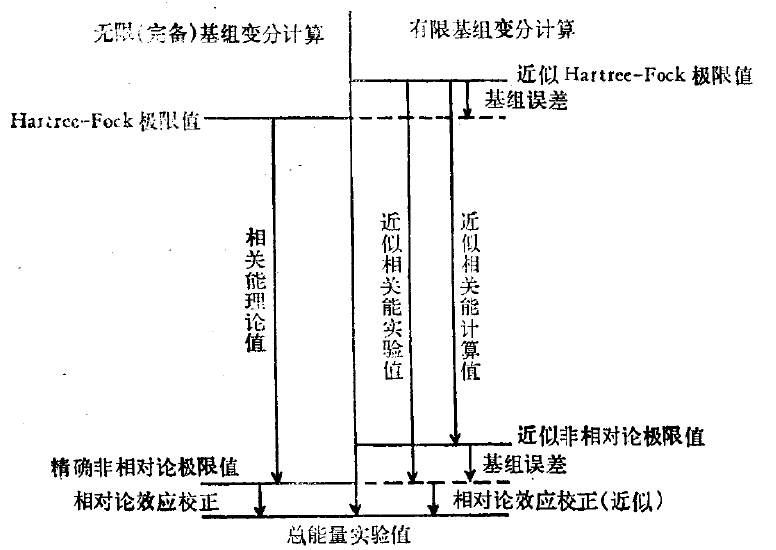
\includegraphics[height=0.42\textwidth,width=0.6\textwidth,viewport=0 0 760 550,clip]{Figures/Post-HF.png}
%\caption{\textrm{ABINIT}的Si.in}
\label{Post-HF}
\end{figure}
}

\frame
{
	\frametitle{\textrm{Post-HF}}
	\textrm{Hartree-Fock}方法精确定义了交换作用,完全没考虑电子相关作用
	\begin{itemize}
		\item \textrm{CI (Configuration Interaction)}
	$$\Psi=\sum_{I=0}C_I\Phi_I=C_0\Phi_0+C_1\Phi_1+C_2\Phi_2+\cdots$$
		\item \textrm{CC (Couple Cluste)}\\
			\begin{displaymath}
				\Psi=\mathrm{e}^{\hat{\mathbf T}}\Phi_0=\mathrm{e}^{(\hat{\mathbf T}_1+\hat{\mathbf T}_2+\hat{\mathbf T}_3+\cdots)}\Phi_0
			\end{displaymath}
		\item \textrm{MP}微扰方法
			\begin{displaymath}
				\begin{aligned}
					&\hat{\mathbf H}=\hat{\mathbf H}^{(0)}+\hat{\mathbf V} \\
					&\hat{\mathbf H}^{(0)}=\sum_i\hat{\mathbf F}_i \qquad \Phi^{(0)}=\Psi_{\mathrm{HF}}\\ 
					&\hat{\mathbf V}=\sum_{j>i}^{\mathrm occ}\dfrac{e^2}{r_{ij}}-\sum_{ij}^{\mathrm occ}\big(\hat{\mathbf J}_{ij}-\dfrac12\hat{\mathbf K}_{ij}\big)
				\end{aligned}
			\end{displaymath}
	\end{itemize}
}

\frame
{
	\frametitle{\rm{Paul Dirac's Commandments}}
	%\textrm{\textcolor{purple}{The fundamental laws necessary for the mathematical treatment of a large part of physics and the whole of chemistry are thus completely known, and the difficulty lies only in the fact that application of these laws leads to equations that are too complex to be solved.}}
\begin{figure}[h!]
\centering
\vspace{-10.5pt}
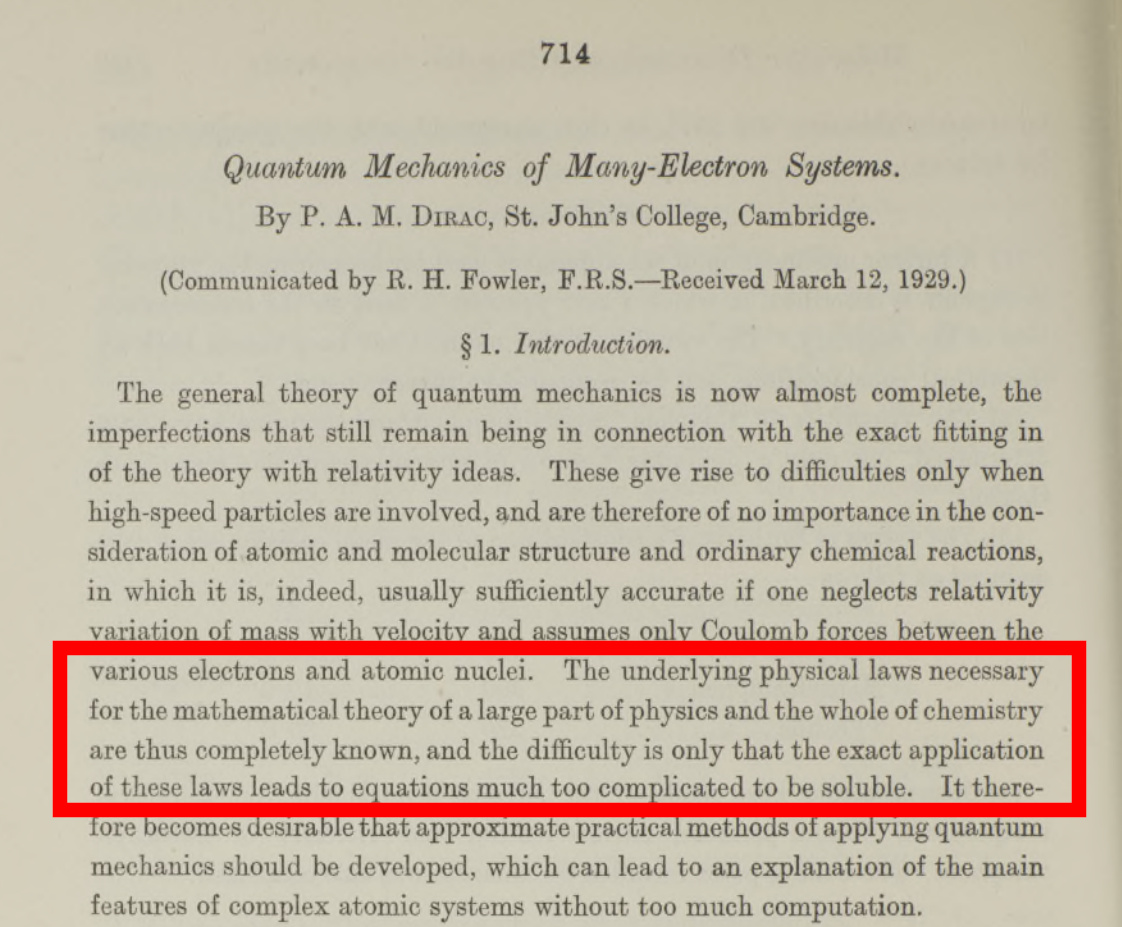
\includegraphics[height=2.7in,width=4.0in,viewport=0 0 1200 890,clip]{Figures/Dirac_comment.png}
\caption{\tiny \textrm{The famous Dirac's commandments.}}%(与文献\cite{EPJB33-47_2003}图1对比)
\label{Dirac_Command}
\end{figure}
}

\section{密度泛函理论}       %Bookmark
\subsection{\rm{Thomas-Fermi~}模型}       %Bookmark
\frame
{
	\frametitle{\textrm{Thomas-Fermi}模型} 
	1927年,\textrm{Thomas}和\textrm{Fermi}基于均匀电子气模型上建立\textrm{Thomas-Fermi}模型,\textcolor{blue}{体系能量可用}\textcolor{red}{电子密度}\textcolor{blue}{表示}:
	\begin{itemize}
		\item 动能表达式
			$$T_{\mathrm{TF}}[\rho(\vec r)]=\dfrac3{10}(3\pi^2)^{\frac23}\int\rho^{\frac53}(\vec r)\mathrm{d}\vec r$$
		\item 外势$V_{ext}(\vec r)$下电子体系的能量泛函表达式为
			\begin{displaymath}
				\begin{aligned}
					E_{\mathrm{TF}}[\rho(\vec r)]=&\dfrac3{10}(3\pi^2)^{\frac23}\int\rho^{\frac53}(\vec r)\mathrm{d}\vec r\\
					&+\int\rho(\vec r)V_{ext}(\vec r)\mathrm{d}\vec r+\dfrac12\int\int\dfrac{\rho(\vec r_1)\rho(\vec r_2)}{|\vec r_2-\vec r_1|}\mathrm{d}\vec r_1\mathrm{d}\vec r_2
				\end{aligned}
			\end{displaymath}
		\item \textrm{Thomas-Fermi}模型完全没有考虑电子的交换-相关作用
	\end{itemize}
}

\frame
{
	\frametitle{\textrm{Thomas-Fermi-Dirac}模型} 
	1930年,\textrm{Dirac}将\textrm{Thomas-Fermi}模型修正,用局域密度近似考虑电子交换作用
			\begin{displaymath}
				\begin{aligned}
					E_{\mathrm{TFD}}[\rho(\vec r)]=&\dfrac3{10}(3\pi^2)^{\frac23}\int\rho^{\frac53}(\vec r)\mathrm{d}\vec r+\int\rho(\vec r)V_{ext}(\vec r)\mathrm{d}\vec r\\
					&+\dfrac12\int\int\dfrac{\rho(\vec r_1)\rho(\vec r_2)}{|\vec r_2-\vec r_1|}\mathrm{d}\vec r_1\mathrm{d}\vec r_2-\dfrac34\bigg(\dfrac3{\pi}\bigg)^{\frac13}\int\rho^{\frac43}(\vec r)\mathrm{d}\vec r
				\end{aligned}
			\end{displaymath}
			\begin{itemize}
				\item 在总电子数守恒约束条件
					$$\int\rho(\vec r)\mathrm{d}\vec r=N$$
					下,能量泛函$E_{\mathrm{TFD}}[\rho(\vec r)]$对密度$\rho(\vec r)$的变分极小获得体系的基态密度和基态能量
			\end{itemize}
}

\frame
{
	\frametitle{\textrm{Thomas-Fermi}模型}
	\begin{itemize}
		\item \textrm{Thomas-Fermi}模型用电子密度代替波函数描述问题是极大的简化,但模型过于粗糙:\\
%			\begin{enumerate}
%				\item 以均匀电子气的密度得到动能的表达式
%				\item 完全忽略电子间的交换-相关作用
%			\end{enumerate}
			不能正确描述相互作用电子体系的基本特征,如原子的壳层结构
		\item \textrm{Thomas-Fermi}模型虽不够精确,但可以通过引入修正项校正:
			\textrm{Dirac}交换泛函 $$E_X[\rho(\vec r)]=-\dfrac34\bigg(\dfrac3{\pi}\bigg)^{\frac13}\int\rho^{\frac43}(\vec r)\mathrm{d}\vec r$$
			\textrm{Wigner}相关泛函 $$E_C[\rho(\vec r)]=-0.056\int\dfrac{\rho^{\frac43}(\vec r)}{0.079+\rho^{\frac13}(\vec r)}\mathrm{d}\vec r$$
	\end{itemize}
	\textrm{Thomas-Fermi}模型为密度泛函理论\textrm{(DFT)}提供了重要的启示
}

\subsection{密度泛函理论}       %Bookmark
\frame                               %
{
\frametitle{密度泛函理论(\textrm{DFT})} %Slide Page Title
%   \secname
与传统的量子力学方法不同,密度泛函理论的基本变量是体系的基态电子密度。%通过体系的电子密度而非波函数确定体系的基态能量。
\begin{itemize}%[+-| alert@+>]
	\item 密度泛函理论的基石:\textrm{Hohenberg-Kohn}定理\upcite{PR136-B864_1964}
\vskip 5pt
\begin{itemize}%[+-| alert@+>]
   \setlength{\itemsep}{8pt}
 \item $E[\rho]=F_{\mathrm{HK}}[\rho]+\displaystyle\int\rho(\vec{r})v(\vec{r})\textrm{d}\vec{r}$ \\
\vskip 5pt 其中$F_{\mathrm{HK}}[\rho]=\underset{\Psi\to\rho}{\mathrm{Min}}\langle\Psi[\rho]|\hat{T}+\hat{W}|\Psi[\rho]\rangle$
是普适的泛函表达式。%,指明多电子体系的基态性质与基态密度间存在一一对应关系
     \textrm{\small{第一定理表明多电子体系的性质完全由体系的基态密度决定}}
   \item 如果$\tilde\Psi\neq\Psi$,
     $E[\tilde\rho]\geqslant E[\rho_0]$\\
     \textrm{\small{第二定理指出基态总能量泛函在体系基态电子密度处取极小值}}
   \end{itemize}
%\textrm{\small{第二定理指出基态总能量泛函在体系基态电子密度处取极小值}}
\vskip 8pt
 \item 密度泛函理论的优越性:用密度($\rho$)代替波函数($\Psi$)描述体系
\vskip 5pt
 \item 密度泛函理论的困难:能量密度泛函的精确形式未知
   \end{itemize}
}

\frame                               %
{
\frametitle{密度泛函理论(\textrm{DFT})}
\textrm{Kohn-Sham}方程\upcite{PR140-A1133_1965}:无相互作用体系+交换-相关能的贡献
$$(T_S+V_{e\!f\!f})|\varphi_i\rangle=\varepsilon_i|\varphi_i\rangle,\quad i=1,\cdots,N,\cdots$$
其中$T_S=-\dfrac12\nabla^2$~~是无相互作用体系的动能
\begin{displaymath}
	\begin{aligned}
		V_{e\!f\!f}(\vec r)=&V_{ext}(\vec r)+\displaystyle\int w(\vec r,\vec r\,')\rho(\vec r\,')\mathrm{d}\vec r\,'+V_{\mathrm{XC}}[\rho]\\
=&\displaystyle\int\dfrac{\rho(\vec r\,')}{|\vec r-\vec r^{\prime}|}\mathrm{d}\vec r\,'+V_{ext}(\vec r)+V_{\mathrm{XC}}[\rho]
	\end{aligned}
\end{displaymath}
$V_{ext}(\vec r)$是电子体系与外部的电荷或磁场相互作用\\
$V_{\mathrm{XC}}[\rho]=\dfrac{\delta E_{\mathrm{XC}}}{\delta\rho(\vec r)}$称为交换-相关势
\vskip 10pt
\textrm{Kohn-Sham}方程是形式上的单粒子方程
\vskip 6pt
\textrm{Kohn-Sham}方程的实质:\\\textcolor{red}{将动能泛函的主要部分分离出来,剩余部分放在交换-相关能中}
}

\frame
{
\frametitle{交换-相关能与交换-相关势}
实际考虑交换-相关能时,会将交换-相关能表示为交换能和相关能之和:
\begin{displaymath}
	E_{\mathrm{XC}}[\rho]=E_{\mathrm{X}}[\rho]+E_{\mathrm{C}}[\rho]=\int\varepsilon_{\mathrm{X}}[\rho]\rho(\vec{r}) \textrm{d}^3\vec{r}+\int\varepsilon_{\mathrm{C}}[\rho]\rho(\vec{r}) \textrm{d}^3\vec{r}
\end{displaymath}
$\varepsilon_{\mathrm{X}}[\rho]$和$\varepsilon_{\mathrm{C}}[\rho]$可理解为单电子的交换能和相关能
\vskip 20pt
交换-相关势通过交换-相关能计算得到:~
		\begin{displaymath}
			V_{\mathrm{XC}}^{\sigma}[\rho_{\alpha},\rho_{\beta}]=\dfrac{\delta E_{\mathrm{XC}}[\rho_{\alpha},\rho_{\beta}]}{\delta\rho_{\sigma}}=\dfrac{\delta\{E_{\mathrm{X}}[\rho_{\alpha},\rho_{\beta}]+E_{\mathrm{C}}[\rho_{\alpha},\rho_{\beta}]\}}{\delta\rho_{\sigma}}
		\end{displaymath}
		\textcolor{red}{注意}:~由于$E_{\mathrm{XC}}[\rho_{\sigma}]$对$\rho_{\sigma}$是非线性的\\
		\textcolor{blue}{$V_{\mathrm{XC}}=V_{\mathrm{X}}+V_{\mathrm{C}}$和$\varepsilon_{\mathrm{XC}}=\varepsilon_{\mathrm{X}}+\varepsilon_{\mathrm{C}}$不同,不要混淆这两个量}
}
%  \beamertemplateshadingbackground{blue!10}{yellow!10}

\frame                               %
{
\frametitle{交换-相关能密度泛函}
\textcolor{blue}{密度泛函理论的核心问题}:\\
\textrm{Kohn-Sham}方程用于实际计算,必须知道$E_{XC}[\rho]$或者$V_{XC}[\rho]$与$\rho(\vec r)$的泛函关系
\vskip 15pt
\begin{minipage}[b]{0.59\textwidth}
 \hspace*{-15pt}
 \begin{itemize}%[+-| alert@+>]
	 \setlength{\itemsep}{10pt}
 \fontsize{7.5pt}{6.0pt}\selectfont{
 \item \textrm{LDA}:泛函只与密度分布的局域值有关
 \item \textrm{GGA}:泛函依赖:局域密度及其梯度
 \item $meta$-\textrm{GGA}:泛函依赖的变量还有动能密度
 \item 杂化(\textrm{hybrid})泛函:泛函与占据轨道有关
 \item 其他的交换-相关能泛函
 \item<1-> 完全非局域泛函:理想泛函,不现实
}
 \end{itemize}
\end{minipage}
\hfill
\begin{minipage}[b]{0.39\textwidth}
\hspace*{-10pt}
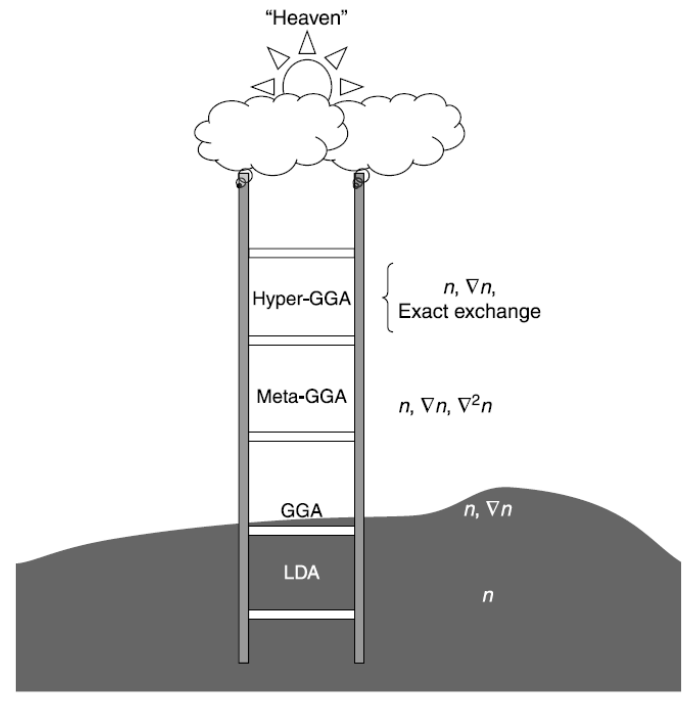
\includegraphics[height=1.7in,width=3.18in,viewport=10 5 1380 700,clip]{Figures/Jacobi-ladder.png}\\
\centering{\textcolor{red}{\textrm{\tiny Jacob's ladder}}}
\end{minipage}
% \begin{itemize}%[+-| alert@+>]
%\item 交换-相关能密度泛函
}

\frame                               %
{
	\frametitle{近似能量泛函$E_{\mathrm{XC}}[\rho]$的主要问题}
\vskip 20pt
\begin{enumerate}%[+-| alert@+>]
   \setlength{\itemsep}{10pt}
 \item  密度是整体变量:~电子自相互作用抵消不净\\%\quad\textrm{(LDA+U)}方法的校正%(\textrm{LDA+U})
	 用\textrm{DFT}计算电子数很少的体系,一般都会有较大的误差
 \item  电子相关:~简并和近简并基态的表示不合理\\
	 基态电子密度用不同的简并轨道计算时,体系能量应保持不变,但现有的近似能量泛函不具有这个性质
 \item  渐近行为:~处理弱相互作用体系的误差大\\
	 如\textrm{Van der Waals}相互作用和现有近似能量泛函本身的计算误差在同一量级
 \end{enumerate}
}

\frame                               %
{
	\frametitle{\textrm{Kohn-Sham}方程}
\begin{figure}[h!]
\centering
\vspace*{-0.21in}
\hspace*{-0.1in}
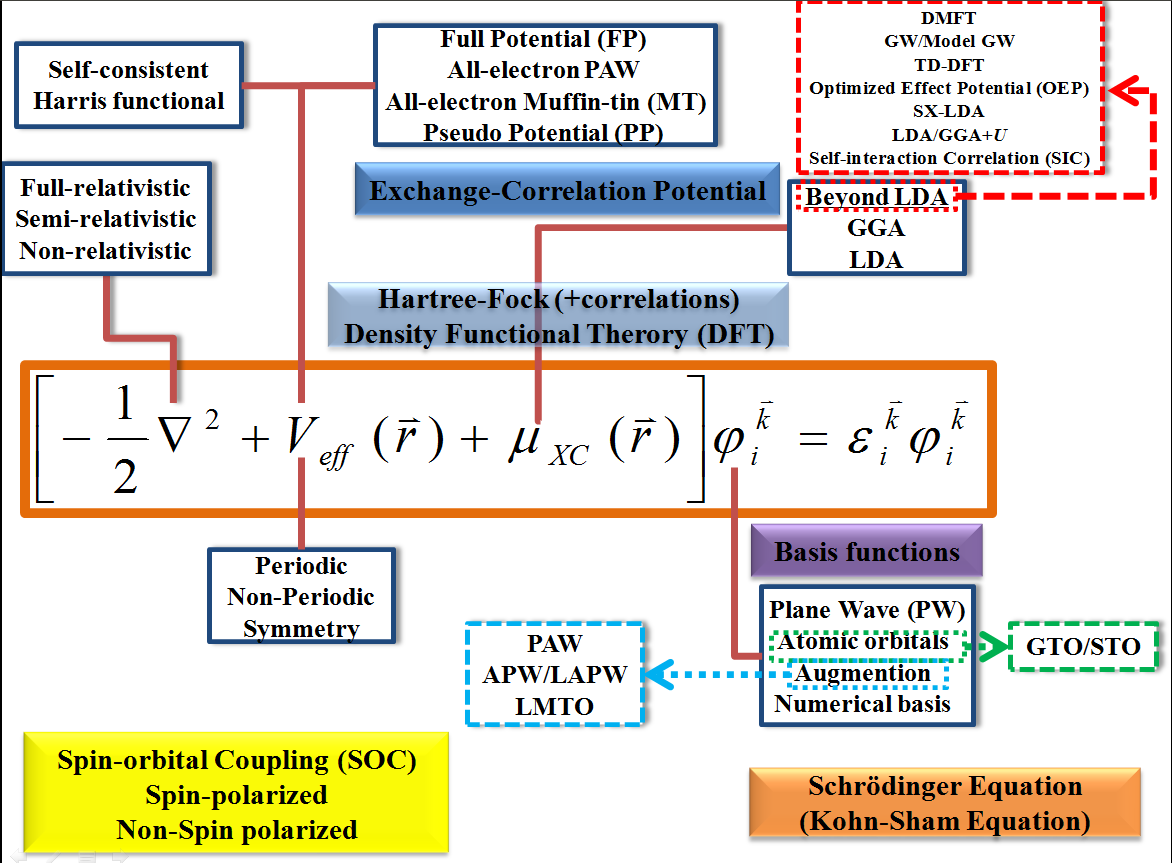
\includegraphics[height=2.7in,width=4.0in,viewport=2 5 1162 880,clip]{Figures/DFT.png}
\caption{\tiny \textrm{The Analysis of Kohn-Sham equation.}}%(与文献\cite{EPJB33-47_2003}图1对比)
\label{DFT}
\end{figure}
}

\frame
{
	\frametitle{\textrm{DFT-SCF}}
\begin{figure}[h!]
\centering
\vspace*{-0.25in}
\hspace*{-0.80in}
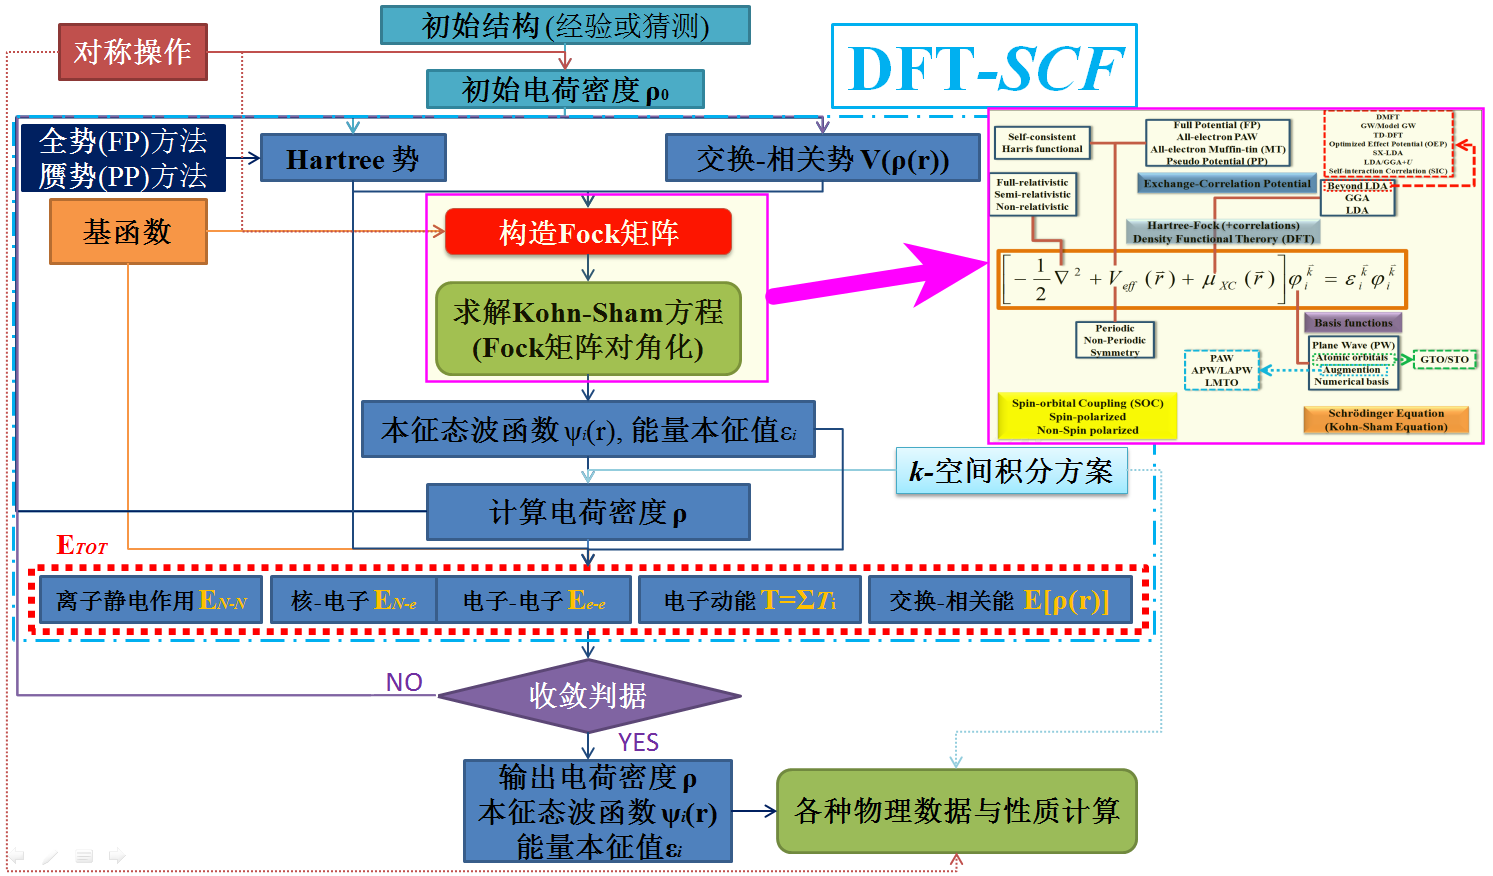
\includegraphics[height=2.80in,width=4.95in,viewport=5 3 1490 870,clip]{Figures/DFT-SCF_2.png}
%\caption{\tiny \textrm{Pseudopotential for metallic sodium, based on the empty core model and screened by the Thomas-Fermi dielectric function.}}%(与文献\cite{EPJB33-47_2003}图1对比)
\label{DFT-SCF-2}
\end{figure}
}
%------------------------------------------------------------------------Reference----------------------------------------------------------------------------------------------
\begin{thebibliography}{99}
\frame[allowframebreaks]
{
\frametitle{主要参考文献}
{\tiny
\bibitem{Xu_Li_Wang}徐光宪、黎乐民、王德民, {\textit{量子化学——基本原理和从头计算法}}\;\textrm{({\textit{上、中}})}\:科学出版社, 北京, 1980
\bibitem{PR136-B864_1964}\textrm{P. Hohenberg and W. Kohn, \textit{Phys. Rev.} \textbf{136} (1964), B864}
\bibitem{PR140-A1133_1965}\textrm{W. Kohn and L.J. Sham, \textit{Phys. Rev.} \textbf{140} (1965), A1133}
\bibitem{PRL49-1691_1982}\textrm{P. Perdew, R. G. Parr, M. Levy and J. L. Balduz, Jr., \textit{Phys. Rev. Lett.} \textbf{49} (1982), 1691}
\bibitem{Parr_Yang}\textrm{R.G. Parr and W. Yang. \textit{Density-Functional Theory of Atoms and Molecules} (Oxford University Press, New York, U.S.A., 1989)}
}
\nocite*{}
}
\end{thebibliography}

%-----------------------------------------------------------------------------
